\documentclass[11pt,a4paper,oldfontcommands,oneside]{memoir}
\usepackage[utf8]{inputenc}
\usepackage{microtype}
\usepackage[dvips]{graphicx}
\usepackage{xcolor}
\usepackage{times}
\usepackage{graphicx}
\usepackage[spanish]{babel}
\usepackage[
breaklinks=true,colorlinks=true,
%linkcolor=blue,urlcolor=blue,citecolor=blue,% PDF VIEW
linkcolor=black,urlcolor=black,citecolor=black,% PRINT
bookmarks=true,bookmarksopenlevel=2]{hyperref}

\usepackage{geometry}
% PDF VIEW
% \geometry{total={210mm,297mm},
% left=25mm,right=25mm,%
% bindingoffset=0mm, top=25mm,bottom=25mm}
% PRINT
\geometry{total={210mm,297mm},
left=20mm,right=20mm,
bindingoffset=10mm, top=25mm,bottom=25mm}

\OnehalfSpacing
%\linespread{1.3}

%%% CHAPTER'S STYLE
\chapterstyle{bianchi}
%\chapterstyle{ger}
%\chapterstyle{madsen}
%\chapterstyle{ell}
%%% STYLE OF SECTIONS, SUBSECTIONS, AND SUBSUBSECTIONS
\setsecheadstyle{\Large\bfseries\sffamily\raggedright}
\setsubsecheadstyle{\large\bfseries\sffamily\raggedright}
\setsubsubsecheadstyle{\bfseries\sffamily\raggedright}


%%% STYLE OF PAGES NUMBERING
%\pagestyle{companion}\nouppercaseheads 
%\pagestyle{headings}
%\pagestyle{Ruled}
\pagestyle{plain}
\makepagestyle{plain}
\makeevenfoot{plain}{\thepage}{}{}
\makeoddfoot{plain}{}{}{\thepage}
\makeevenhead{plain}{}{}{}
\makeoddhead{plain}{}{}{}


\maxsecnumdepth{subsection} % chapters, sections, and subsections are numbered
\maxtocdepth{subsection} % chapters, sections, and subsections are in the Table of Contents


%%%---%%%---%%%---%%%---%%%---%%%---%%%---%%%---%%%---%%%---%%%---%%%---%%%

\begin{document}

%%%---%%%---%%%---%%%---%%%---%%%---%%%---%%%---%%%---%%%---%%%---%%%---%%%
%   TITLEPAGE
%
%   due to variety of titlepage schemes it is probably better to make titlepage manually
%
%%%---%%%---%%%---%%%---%%%---%%%---%%%---%%%---%%%---%%%---%%%---%%%---%%%
\thispagestyle{empty}

{%%%
\sffamily
\centering
\Large

~\vspace{\fill}

\includegraphics[scale=1]{logo.png} \\
{\huge 
\vspace{4cm}
Describir la parametrización de rotaciones de acuerdo a los ángulos de Euler
}
\vspace{2.5cm}

{\LARGE
Eduardo Robles Vázquez
}

\vspace{2.5cm}

Universidad Politécnica de la Zona Metropolitana de Guadalajara

\vspace{3.5cm}

Profesor: Carlos Enrique Morán Garabito

\vspace{\fill}

08 de Octubre de 2019

%%%
}%%%

\vspace{.5cm}
\hfill\break




\tableofcontents*

\clearpage

%%%---%%%---%%%---%%%---%%%---%%%---%%%---%%%---%%%---%%%---%%%---%%%---%%%
%%%---%%%---%%%---%%%---%%%---%%%---%%%---%%%---%%%---%%%---%%%---%%%---%%%
\chapter{Introducción}
El movimiento general de un sólido rígido posee 6 grados de libertad.
Por el teorema de Chasles, el movimiento general de un sólido puede descomponerse en una traslación de un punto seguida de una rotación del sólido alrededor de este punto (es decir, tomándolo como fijo en la rotación). Por ello, en la parametrización del movimiento de un sólido, estos 6 grados pueden descomponerse en 3 de traslación y tres de rotación.\\
Como grados de libertad de traslación basta dar el desplazamiento de un punto concreto del sólido (centro de reducción).
Para la rotación, en cambio, existen diferentes formas de parametrizarla, cada una con sus ventajas e inconvenientes. Así, tenemos:\\


1.	Dar directamente la matriz de rotación que pasa de un sistema de referencia ligado al sólido a uno exterior tomado como fijo. Esta matriz tiene 9 elementos sometidos a seis vínculos, lo cual multiplica el número de ecuaciones necesarias para la descripción del movimiento.\\

2.	Dar la orientación del eje de giro mediante dos ángulos (que pueden ser coordenadas esféricas, como la latitud y la longitud) y el ángulo de giro alrededor de este eje. Tiene el inconveniente, como los ángulos de Euler y otros, que requieren un abundante uso de funciones trigonométricas.\\

3.	Emplear los denominados parámetros de Euler que son un conjunto de cuatro variables, con un vínculo, que permiten representar toda matriz de rotación. Vienen a ser la generalización a 3 dimensiones de usar x e y para dar una rotación en el plano, sujetas a la condición x2 + y2 = 1. Tienen el inconveniente de que no son fáciles de visualizar, aunque computacionalmente son muy eficientes.\\

4.	Emplear otros parámetros, como los de Cailey-Klein, que representan las rotaciones como operaciones sobre números complejos.\\

5.	Escribir la rotación general como una composición de tres rotaciones individuales sobre diferentes ejes. Esta es la técnica que se usa para definir los ángulos de Euler y los ángulos de navegación (o de Tait-Bryan). La diferencia entre los de Euler y los de Tait-Bryan es que en el primer caso se repite uno de los ejes, y en el segundo los tres ejes son diferentes. 

\chapter{Ángulos de Euler}
Puede demostrarse que cualquier rotación de un sólido puede expresarse como la composición de tres rotaciones elementales alrededor de ejes diferentes. A su vez, estas rotaciones pueden considerarse en torno a unos ejes fijos o en torno a unos ejes intrínsecos. Aquí consideraremos la segunda opción, es decir, especificaremos una composición de rotaciones que nos llevarán desde un sistema exterior considerado fijo (sólido 1) hasta un sistema ligado al sólido (sólido 4) mediante sólidos intermedios. Para ello: \\ \\
1.	Primero efectuamos una rotación de un ángulo en torno a un eje del sólido 1 que nos lleva a un sólido intermedio 2.\\
2.	A continuación, rotamos un ángulo en torno a un eje del sólido 2, que nos lleva a un sólido intermedio 3.\\
3.	Por último, giramos un cierto ángulo en torno a un eje del sólido 3, lo que nos lleva hasta el sólido móvil 4.

\chapter{Posición y matriz de rotación}
Para obtener el resultado de la rotación, debemos ver qué posición ocupa en el sistema de referencia fijo un punto perteneciente al sólido. El vector de posición se escribirá con componentes diferentes en la base fija y en la base móvil, aunque el vector sea el mismo donde, por ser un punto del sólido las componentes (X, Y, Z) son constantes. El problema se reduce entonces a relacionar los vectores de las bases. Para ello, componemos las tres rotaciones. En las siguientes imágenes se ve las rotaciones gráficamente (figura 1.0 y la figura 1.2).

\begin{center}
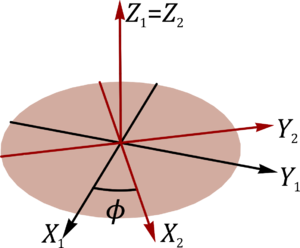
\includegraphics[scale=2.5]{Angulos.png} 
\\
Figura 1.0
\end{center}

\begin{center}
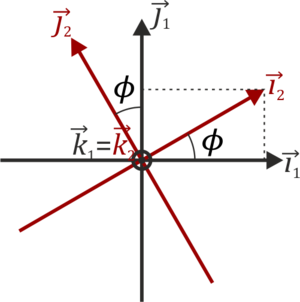
\includegraphics[scale=2.5]{grafica.png} 
\\
Figura 1.2
\end{center}

La primera rotación es una de un ángulo $\phi$, en torno al eje $OZ_1 = OZ_2$, que nos lleva al sólido 2. La relación entre la base fija 1 y la intermedia 2 es:

\begin{center}
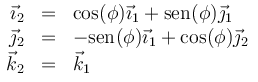
\includegraphics[scale=1.5]{1.png} 
\end{center}

Siendo su relación inversa:

\begin{center}
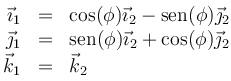
\includegraphics[scale=1.5]{2.png} 
\end{center}

A esta rotación, cuando se realiza sin modificar ninguno de los otros dos ángulos, se la denomina movimiento de precesión.

\section{Nutación}
La segunda rotación consiste en el giro de un ángulo $\theta$ alrededor del eje $OX_2 = OX_3$. A este eje, que no se ve modificado por la rotación, se lo denomina línea de nodos. Esta rotación nos lleva al sólido intermedio 3, cuya base se relaciona con la 2 por:

\begin{center}
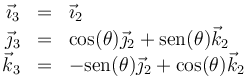
\includegraphics[scale=1.5]{3.png} 
\end{center}

Siendo su relación inversa:

\begin{center}
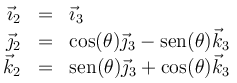
\includegraphics[scale=1.5]{4.png} 
\end{center}

Cuando se produce esta rotación sin que se modifiquen las otras dos se dice que el sólido efectua un movimiento de nutación.\\

Gráficamente se pueden visualizar en la Figura 2.0 y 2.1

\begin{center}
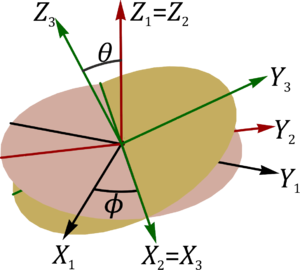
\includegraphics[scale=3.1]{3D.png} 
\\
Figura 2.0
\end{center}

\begin{center}
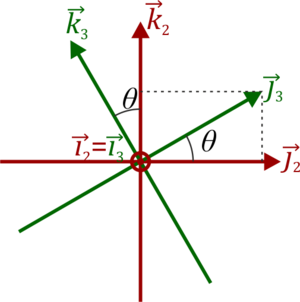
\includegraphics[scale=3.0]{plano.png} 
\\
Figura 2.1
\end{center}

\section{Rotación propia}
El tercer giro (rotación propia) corresponde a un nuevo giro de un ángulo alrededor del ángulo $OZ_3 = OZ_4$ (que no es el mismo, normalmente, que el $OZ_1 = OZ_2$). La relación entre las bases 3 y 4 es análoga a la que hay entre la 1 y la 2.

\begin{center}
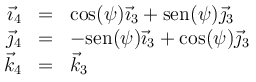
\includegraphics[scale=1.5]{5.png} 
\end{center}

Siendo su relación inversa:

\begin{center}
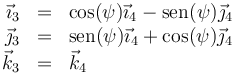
\includegraphics[scale=1.5]{6.png} 
\end{center}

Como se muestra en la figura 3.0 y 3.1
\begin{center}
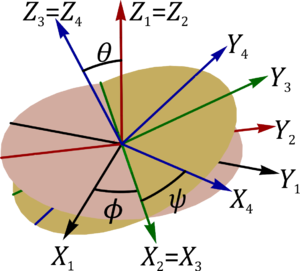
\includegraphics[scale=2.5]{x.png} 
\\
Figura 3.0
\end{center}
\begin{center}
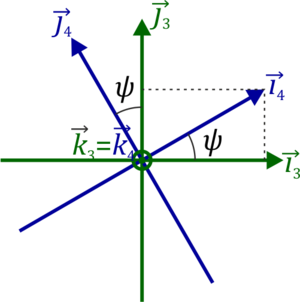
\includegraphics[scale=2.5]{j.png} 
\\
Figura 3.1
\end{center}

El origen de los nombres precesión, nutación y rotación procede del análisis del movimiento terrestre. La rotación es el movimiento alrededor del eje terrestre. La precesión es el lento movimiento de dicho eje. La nutación es el cambio en la inclinación del eje terrestre.


\bibliographystyle{plain}
\bibliography{bibliografia}


\end{document}

